%LaTeX SAMPLE FILE FOR PAPERS OF CDAM

% LaTeX 2e
\documentclass[12pt]{article}

\usepackage{graphicx}
\usepackage{epsfig}
\usepackage{cite}
\usepackage{amsmath,amssymb,amsfonts,amsthm}
\usepackage[boxed]{algorithm2e}
\usepackage{caption}
\usepackage{wrapfig}
\usepackage{upgreek}
\usepackage{adjustbox}
\usepackage{pbox}
\usepackage{index}
\usepackage{color}
\usepackage{makecell}
\usepackage{multirow}
\usepackage{bbm}
\usepackage{lastpage}
\usepackage{longtable}
\usepackage{changepage}

% LaTeX 2.09
%\documentstyle[12pt]{article}

%%%%%%%%%%%%%%%%%%%%%%%%%%%% paper layout %%%%%%%%%%%%%%%%%%%%%%%%%%%%%%
\hoffset=-1in
\voffset=-1in
% Please, don't change this layout
\parindent=6mm
\topskip=0mm
\topmargin=30mm
\oddsidemargin=27.5mm
\evensidemargin=27.5mm
\textwidth=155mm
\textheight=237mm
\headheight=0pt
\headsep=0pt
\footskip=2\baselineskip
\addtolength{\textheight}{-\footskip}

\providecommand{\keywords}[1]
{
\vspace{2mm}\hspace{20pt}\textbf{\textit{Keywords:}} #1
}

\providecommand{\abskeyw}[2]
{
\begin{small}
\begin{adjustwidth}{10mm}{10mm}
\vspace{1mm}\hspace{20pt}#1

\keywords{#2}
\end{adjustwidth}
\end{small}
}

% To remove after translation
%\usepackage[T2A]{fontenc}
%\usepackage[utf8]{inputenc}
\usepackage[english]{babel}
\usepackage{bm}

\begin{document}

%%% Title section
\begin{center}
{\Large\bf Monte Carlo SSA for extracting weak signals}\\\vspace{2mm} {\sc E. Poteshkin$^1$, N. Golyandina$^2$}\\\vspace{2mm}
{\it $^{1}$ $^{2}$St.Petersburg State University\\
%$^{2}$Institute  ...\\
St.Petersburg, Russia\\} e-mail: {\tt $^1$egor.poteshkin@yandex.ru,
$^2$n.golyandina@spbu.ru}

\abskeyw{The paper addresses the issue of extracting signals from noise using singular spectrum analysis (SSA). We propose an algorithm that automatically selects significant modulated harmonics without specifying their periods. This algorithm is based on the Monte Carlo SSA criterion and determines and then extracts the significant frequencies.}{time series, signal extraction, signal detection, singular spectrum analysis}
\end{center}

\section{Introduction}

Consider the following model: $\mathsf{X}=\mathsf{S}+\mathsf{R}$, where $\mathsf{X} = (x_1,\ldots,x_N)$ is the observed time series, $\mathsf{S}$ is the signal and $\mathsf{R}$ is the noise, i.e., the realisation of some stationary process.  This paper considers two problems: signal detection and signal extraction in cases where the signal is present.

To solve the first problem, we use the Monte Carlo SSA (MC-SSA)~\cite{AllenSmith96} method, which tests the hypothesis $H_0:\mathsf{S}=0$. The second problem is solved by applying singular spectrum analysis (SSA)~\cite{Broomhead1986, ssa2001}, which decomposes the series into elementary components. After grouping these components, we obtain a decomposition of the series into trend, periodic components, and noise.   As one of the SSA steps involves visual analysis to identify the signal components, there is a need to automate this step. This problem has been addressed in works such as~\cite{alexandrov, Kalantari2019, circSSA, autoSSA}, which are mainly devoted to trend extraction or smoothing. This paper aims to define an approach to the automatic extraction of weak oscillating signals detected by the MC-SSA criterion.

\section{The autoMCSSA algorithm}
Let us introduce some notation and assumptions.

The proposed algorithm uses a modified version of MC-SSA that corrects for multiple comparisons~\cite{Golyandina2023}. Sine waves with equidistant frequencies $\omega_k=k/(2L)$, $k=1,\ldots,L$, were chosen as the projection vectors needed to construct the criterion statistics. With this choice of projection vectors, we can identify significant frequencies present in the signal.

For a series $\mathsf{X}$ of length $N$ and $0\leqslant\omega_1\leqslant\omega_2\leqslant0.5$, we will use the same frequency measure used in~\cite{alexandrov} for trend extraction.
Let the measure $T(\mathsf{X};\omega_1,\omega_2)$ reflect the contribution of frequencies from the interval $[\omega_1,\omega_2)$ calculated from the periodogram of the series.

\begin{figure}[htbp]
    \centering
    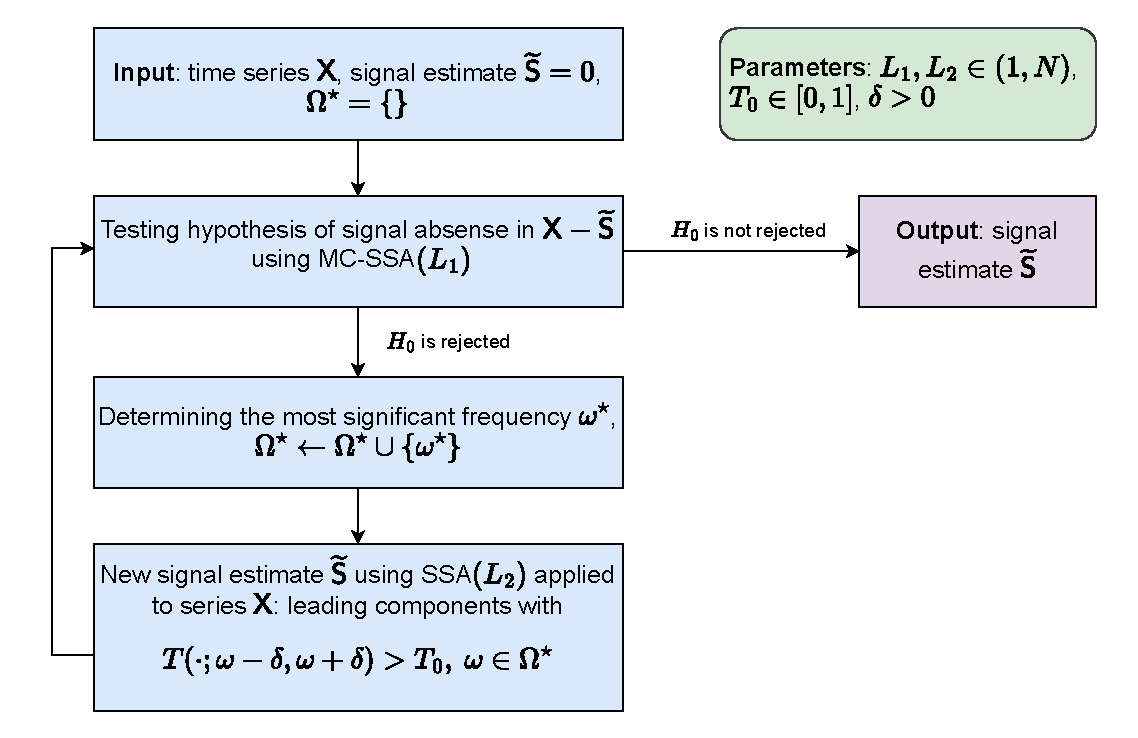
\includegraphics[width=\textwidth]{img/auto_mcssa_alg.pdf}
    \caption{Algorithm autoMCSSA}
    \label{fig:autoMCSSA_alg}
\end{figure}

Figure ~\ref{fig:autoMCSSA_alg} shows the flowchart of the autoMCSSA algorithm. It consists of applying the MC-SSA criterion sequentially until the hypothesis is no longer rejected. If the hypothesis is rejected at the next iteration of the algorithm, the maximum significant frequency $\omega^\star$ is determined and a new signal estimate is calculated using SSA applied to the original series: for each frequency $\omega$, the leading components with a measure $T$ exceeding the threshold $T_0$ are selected from the set of significant frequencies $\Omega^\star$. Once the null hypothesis is no longer rejected, the algorithm terminates, with the final signal estimate being given by$\widetilde{\mathsf{S}}$ .

We will estimate the frequency $\omega^\star$ using a weighted average of the nearest significant frequencies, where the weights are determined by the frequencies' significance.
This estimation method enables us to obtain a more accurate estimate of $\omega$ in the case when it does not fall in the $k/(2L)$ lattice.

Let us consider an example of the work of the considered algorithm. Let $\mathsf{X}=\mathsf{S}+\bm{\xi}$, where $\bm\xi$ is the AR(1) model with parameters $\phi=0.7$ and $\sigma^2=1$, $N=200$, $\mathsf{S}=(s_1,\ldots, s_N)$,
\[
s_n=0.075\, e^{0.02n}\cos(2\pi n/8) + 2\cos(2\pi n / 4) + 0.2\cdot(-1)^n.
\]

\begin{figure}[!h]
    \centering
    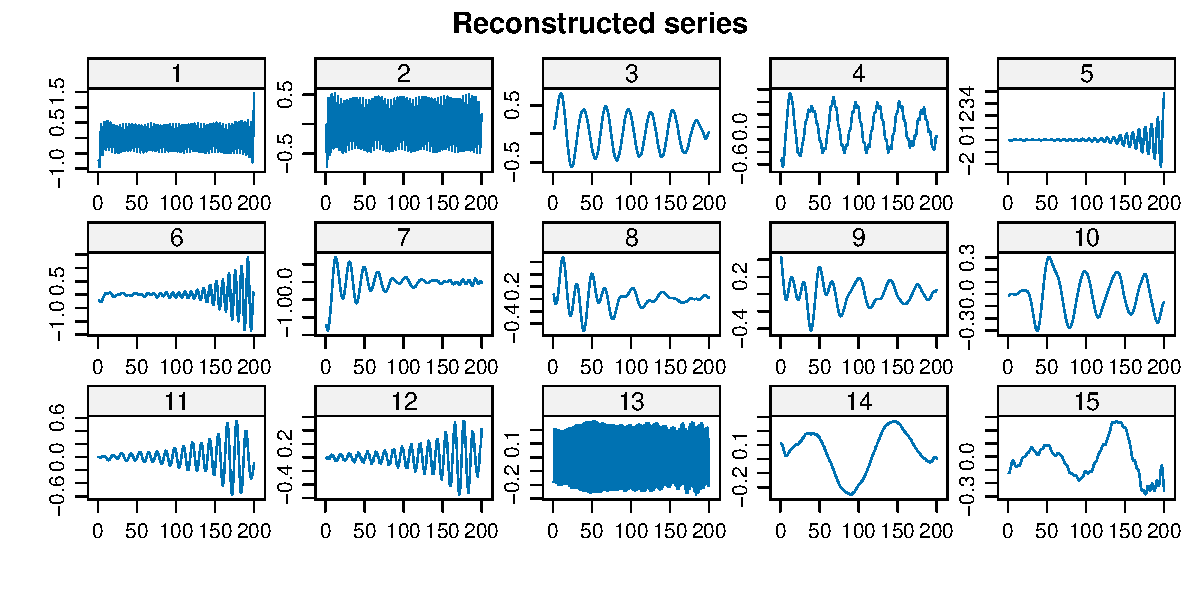
\includegraphics[width=\textwidth]{img/reconstructed_ts.pdf}
    \caption{Elementary series components}
    \label{fig:reconstructed_ts}
\end{figure}

\begin{figure}[!h]
    \centering
    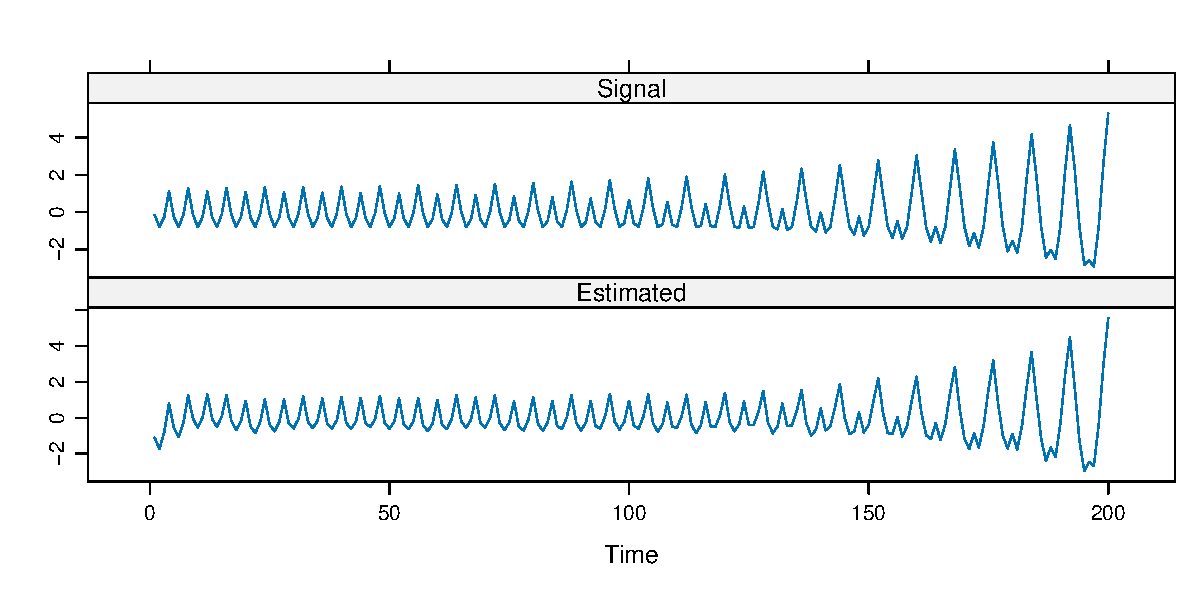
\includegraphics[width=0.8\textwidth]{img/auto_mcssa_result.pdf}
    \caption{Estimated signal using autoMCSSA ($L_1=50$, $L_2=100$, $\delta=1/80$, $T_0=0.5$)}
    \label{fig:autoMCSSA_res}
\end{figure}

Figure~\ref{fig:reconstructed_ts} shows the first $15$ elementary components reconstructed using SSA. The signal corresponds to components with indices $1$, $2$, $5$, $6$, and $13$. Without knowing the formula by which this signal is generated, it is difficult to say with certainty which components are non-random, since the components ($3$, $4$) and ($11$, $12$) look like pairs of harmonics. We applied the autoMCSSA algorithm to this series and found that the developed method correctly identified the components corresponding to the signal. Figure~\ref{fig:autoMCSSA_res} shows the signal $\mathsf{S}$ and its estimation by the autoMCSSA method.

\section{Conclusion}
Thus, the paper proposes an algorithm capable of extracting only the significant components. It is not necessary to specify a period for the periodic component; the periodic components can be multiple and modulated with different amplitude modulation.

%% please make bibitems content in a style below !!!
%% papers with "free style" bibitems content will be rejected !!!

\begin{thebibliography}{10}

    \bibitem{AllenSmith96} Allen~M., Smith~L. Monte Carlo SSA: detecting irregular oscillations in the presence of coloured noise // Journal of Climate.~--- 1996.~--- Vol.~9.~--- P.~3373--3404.
    \bibitem{Broomhead1986} Broomhead~D., King~G. Extracting qualitative dynamics from experimental data // Physica D: Nonlinear Phenomena.~--- 1986.~--- Vol. 20, no. 2–3.~--- P.~217--236.
    \bibitem{ssa2001} Golyandina~N., Nekrutkin~V., Zhigljavsky~A. Analysis of Time Series Structure: SSA and Related Techniques.~--- Chapman and Hall/CRC, 2001.
    \bibitem{alexandrov} Alexandrov Th. A method of trend extraction using singular spectrum analysis // RevStat.~--- 2009~--- Vol.~7 no~1.~--- P.~1-–22.
    .~--- 2004.~--- Vol.~7-80.~--- P.~54--61.
    \bibitem{Kalantari2019} Kalantari~M., Hassani.~H. Automatic grouping in singular spectrum analysis // Forecasting.~--- 2019.~--- Vol. 1, no 1.~--- P.~189--204.
    \bibitem{circSSA} Bogalo~J., Poncela~P., Senra~E. Circulant singular spectrum analysis: A new automated procedure for signal extraction // Signal Processing.~--- 2021.~--- Vol.~179.
    \bibitem{autoSSA} Golyandina~N., Dudnik~P., Shlemov~A. Intelligent Identification of Trend Components in Singular Spectrum Analysis // Algorithms.~--- 2023.~--- Vol. 16.~--- ID 353.
    \bibitem{Golyandina2023} Golyandina~N. Detection of signals by Monte Carlo singular spectrum analysis: multiple testing // Statistics and Its Interface.~--- 2023.~--- Vol.~16. no~1.~--- P.~147--157.

\end{thebibliography}


\end{document}
